\section{Results}
This section contains analysis and results of the planning framework and is subdivided into three subsections: uncontested results, contested results, and multi-rate comparisons.  
\subsection{Baseline and Setup}
The several experiments in this section compare the results of the the framework given in equation \ref{eqn:finalObjective} with a baseline. The baseline attempts to model the general behavior of a stereotypical bus driver. From conversations with the Utah Transit Authority (UTA), bus drivers generally enter the station and top off their bus's battery if a charger is available. The baseline reflects the bus driver behavior with an objetive function which maximizes the number of instances where a bus plugs in. The number of plug-in instances can be computed as the sum of group flow values and results in the objetive function
\begin{equation}
	\underset{\mathbf{y}}{\text{max}} \ \mathbf{1}^TB\mathbf{y},
\end{equation}
\par All other constraints are held equal, resulting in a baseline formulation given as
\begin{equation}\label{eqn:finalBaselineObjective}
	\begin{matrix*}[c]
		\underset{\mathbf{y}}{\scalebox{1}{\text{max}}} \ \mathbf{1}^TB\mathbf{y} \ \text{subject to}\\
		\begin{bmatrix*}[l]
				\tilde{A} \\
				D_{\text{eq}} \\
				P
				\end{bmatrix*} \mathbf{y} = \begin{bmatrix*}[l]\mathbf{c}_f \\ \mathbf{d}_{\text{eq}}\\\mathbf{p} \end{bmatrix*}, \ \begin{bmatrix*}[l]
			\tilde{B} \\
			D_{\text{ineq}} \\ 
			P_{\text{max}} \\
			P_{\text{on}} \\
			P_{\text{off}}
			\end{bmatrix*}\mathbf{y} \le \begin{bmatrix*}\mathbf{1} \\ \mathbf{d}_{\text{ineq}} \\ \mathbf{0} \\ \mathbf{0} \\ \mathbf{0} \end{bmatrix*}
	\end{matrix*}.
\end{equation}
	\par Additionally, each experiment is run in five minute increments such that $t_k$ represents a time instance five minutes behind $t_{k+1}$.  START HERE == was working to find how long for a full charge to justify a bar. will fill in bar charts with this value as well.

\subsection{Uncontested Results}
This section compares the charge schedule associated with equation \ref{eqn:finalObjective} with a schedule developed by a baseline algorithm.  The baseline adheres to all the constraints given previously, but maximizes the objective 
\begin{equation}
	\underset{\mathbf{y}}{\text{max}} \ \mathbf{1}^TB\mathbf{y},
\end{equation}
which incentivizes bus charging when possible. An initial cost comparison is given for an uncontested scenario where the number of chargers is equal to the number of buses. The cost breakdown is given in figure \ref{fig:costComparison}.
\begin{figure}
	\centering
	\makeComparisonBarChart{media/costComparison5Bus5Chargers.csv}{Cost (Dollars)}{Baseline}{Optimized}
	\caption{Cost Comparison between optimized and baseline algorithms}
	\label{fig:costComparison}
\end{figure}
\par Note how the energy charge is equivalent, which indicates that similar amounts of energy were consumed in both scenarios. Dispite the similarity in energy consumption, however, facilities and on-peak power chargers are significantly larger for the unoptimized schedule. 
\par Figure \ref{fig:totalPower1} compares the average power use between the optimized and baseline algorithms. There are two primary differences between the two. The first is that the optimized schedule avoids charging during on-peak hours.  The second is how the optimized charge schedule regulates each charge event to spread the power draw over larger, intermittent periods of time. Avoiding the on-peak time window and minimizing average power draw resulted in the cost disparities shown in figure \ref{fig:costComparison}.

\begin{figure*}
	\centering
	\makeComparisonTotalPower{media/baseline5Bus5ChargerTotalPowerPlot.csv}{media/optimized5Bus5ChargerTotalPowerPlot.csv}{15-Minute Average Power (kW)}{Baseline}{Optimized}
	\caption{15-Minute AVerage Power for one day}
	\label{fig:totalPower1}
\end{figure*} 
Figure \ref{fig:powerPlot1} separates the power draw into power from external loads and power used by buses and shows again how bus charging was optimized to avoid on-peak hours and spread power use over time.  
\begin{figure*}
	\centering
	\makeComparisonPower{media/baseline5Bus5ChargerPowerPlot.csv}{media/optimized5Bus5ChargerPowerPlot.csv}{15-Minute AVerage Power (kW)}{Baseline}{Optimized}
	\caption{Comparison between uncontrolled and bus loads}
	\label{fig:powerPlot1}
\end{figure*}

\subsection{Contested Results}
An optimized schedule can also be produced in resource contested environments. Contention occures when the number of chargers is scarce in comparison to the number of buses and can require that buses charge in disoptimal circumstances.  For example, if charging resources are saturated during off-peak hours, other buses might be forced to charge in the on-peak window. 
\par Figure \ref{fig:contention1} shows the monthly cost from a scenario with one charger and multiple buses. Note the minimial cost increase per bus.  Each subsequent bus incurs a minimal additional cost, showing that charge plans also minimize charge in the presence of contention.
\begin{figure}
	\begin{tikzpicture}
		\begin{axis}[SmallPointPlot, xlabel=Number of Buses, ylabel=Total Monthly Cost, ymin=3000, xmax=11]
			\addplot[blue, only marks, mark size=3pt] coordinates {(5,3034.35) (6,3108.23) (7,3174.54) (8,3255.87) (9,3313.43) (10, 3391.16) (11, 3463.42)}; 
			\addplot[blue] coordinates {(5,3034.35) (6,3108.23) (7,3174.54) (8,3255.87) (9,3313.43) (10, 3391.16) (11, 3463.42)};
		\end{axis}
	\end{tikzpicture}
	\caption{Results for several single charger scenarios.}
	\label{fig:contention1}
\end{figure}
\par Figure \ref{fig:contention2} demonstrates how cost is minimized in the presence of contention. Figure \ref{fig:contention2} compares loads between a 5 and 11 bus scenario, where only one charger is given and the uncontrolled loads are equivalent. In the 5 bus scenario, loads are distributed amongst off-peak hours, resulting in an optimized cost.  The 11 bus scenario requires significantly more power and is forced to charge during on-peak hours.  Note however that average power use is kept relatively low and seldom increases the maximum average power for on-peak use. Both scenarios also make ample use of night charging, where the number of chargers is the same as the number of buses.  
\begin{figure*}
	\centering
	\makeComparisonPower{media/optimized5Bus1ChargerPowerPlot.csv}{media/optimized11Bus1ChargerPowerPlot.csv}{15-Minute AVerage Power (kW)}{5 Bus Scenario}{11 Bus Scenario}
	\caption{Comparison of the loads for a 5 and 11 bus scenario with one overhead charger} 
	\label{fig:contention2}
\end{figure*}

\subsection{Multi-Rate Comparison}
Figure \ref{fig:multiRateCostComparison} shows the comparison between multi and single-rate charging. Both scenarios include 5 buses and 1 charger. As shown in figure \ref{fig:multiRateCostComparison}, the cost difference is marginal at best.  The cost of the multi-rate scenario is \$3006.94 and the cost of the single-rate scenario is \$3007.77. 
\begin{figure}
	\centering
	\makeComparisonBarChart{media/costComparisonMultiVsSingle.csv}{Cost (Dollars)}{Multi-Rate}{Single-Rate}
	\caption{Cost Comparison between a multi-rate and single-rate charge schedule}
	\label{fig:multiRateCostComparison}
\end{figure}
The small cost decrease is also consistent with larger scenarios as shown in figure \ref{fig:costComparisonMultiVsSingleLarge}. 
\par Upon further observation, maximum charge edges in multi-rate scenarios are used more frequently than their low-charge counterparts as shown in figure \ref{fig:chargeRateHistogram}. This would help explain the similarities in cost. If the highest rate is almost always selected, then the resulting plan would resemble a single-rate schedule.  
\begin{figure}
	\makeComparisonBarChart{media/costComparisonMultiVsSingleLarge.csv}{Cost (Dollars)}{Multi-Rate}{Single-Rate}
	\caption{Cost Comaprison between multi and single rate charging for a 35 bus 6 charger scenario}
	\label{fig:costComparisonMultiVsSingleLarge}
\end{figure}
\par Cost is also based on the average instantanous power. Because both single and multi-rate plans charge buses in relatively small time periods the average power use is kept relatively low (see figures \ref{fig:contention2}, and \ref{fig:contention1}). There are also many circumstances when a bus's charge time is limited, resulting in high charge rates.
\begin{figure}
	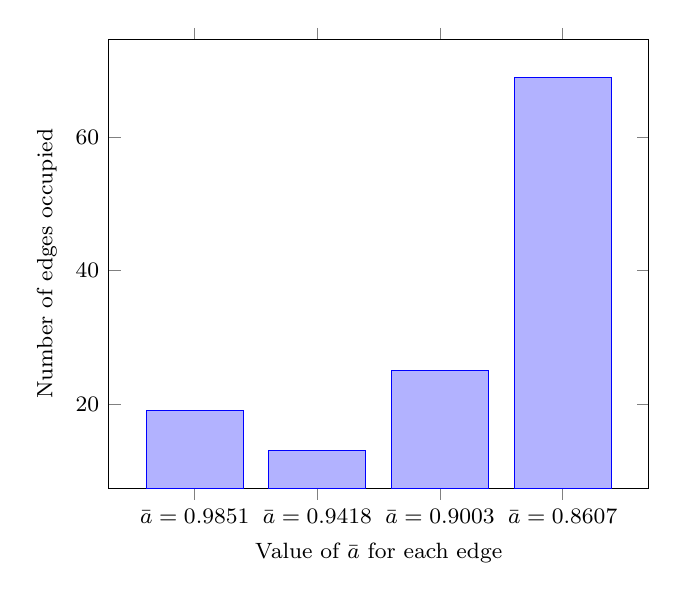
\begin{tikzpicture}
		\begin{axis}[ybar, xmin=0.3, xmax=4.7, font=\footnotesize, xtick={1,2,3,4},xticklabels={$\bar{a} = 0.9851$,$\bar{a} = 0.9418$,$\bar{a} = 0.9003$,$\bar{a} = 0.8607$},
			xlabel=Value of $\bar{a}$ for each edge, ylabel=Number of edges occupied, bar width=35pt]
			\addplot coordinates{(1,19) (2,13) (3,25) (4,69)};
		\end{axis}
	\end{tikzpicture}
	\caption{Histogram of charge rates}
	\label{fig:chargeRateHistogram}
\end{figure}













